\objectives{%
      \item compute and conceptually distinguish training and testing misclassification errors
      \item explain how the problem of achieving low testing error
            decomposes into the three problems of achieving low
            \emph{generalization},
            \emph{optimization}, and
            \emph{approximation}
            errors.
}

\sampassage{error analysis}
  Intuitively, our testing error of $17\%$ comes from three sources:
  \textbf{(a)} the failure of our training set to be representative of our testing set;
  \textbf{(b)} the failure of our program to exactly minimize training error over $\hH$; and
  \textbf{(c)} the failure of our hypothesis set $\hH$ to contain ``the true'' pattern.

  These are respectively errors of
  \textbf{generalization},
  \textbf{optimization},
  \textbf{approximation}.

  We can see generalization error when we plot testing data in the
  brightness-width plane.  The hypotheses $h=(20, 83)$ that we selected based
  on the training in the brightness-width plane misclassifies many testing
  points.  we see many misclassified points.  Whereas $h$ misclassifies only
  $10\%$ of the training data, it misclassifies $17\%$ of the testing data.
  This illustrates generalization error.

  In our plot of the $(a,b)$ plane,
  the {\blu blue square} is the hypothesis $h$ (in $\hH$) that best fits
  the training data.  The {\rng orange square} is the hypothesis (in
  $\hH$) that best fits the testing data.  But even the latter seems
  suboptimal, since $\hH$ only includes lines through the origin while it
  seems we want a line --- or curve --- that hits higher up on the
  brightness axis.  This illustrates approximation error.\bovinenote{%
    To define \emph{approximation error}, we need to specify whether the `truth'
    we want to approximate is the training or the testing
    data.  Either way we get a useful concept.  In this paragraph we're talking
    about approximating \emph{testing} data; but in our notes overall we'll
    focus on the concept of error in approximating \emph{training} data.
  }

  Optimization error is best seen by plotting training rather than testing
  data.  It measures the failure of our selected hypothesis $h$ to minimize
  training error --- i.e., the failure of the {\blu blue square} to lie in a
  least shaded point in the $(a,b)$ plane, when we shade according to training
  error.

  \begin{figure}[h]
  %\begin{marginfigure}%[h]
      \centering
      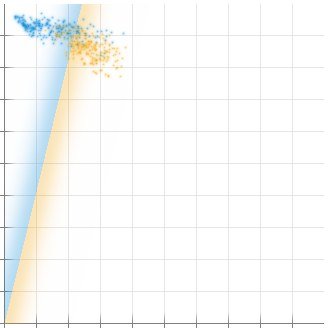
\includegraphics[width=0.49\textwidth]{example-mnist/test-features.png}%
      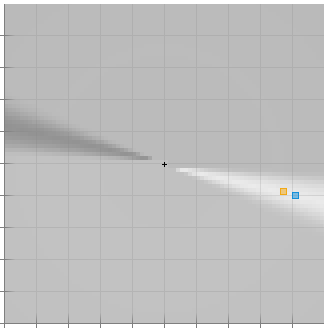
\includegraphics[width=0.49\textwidth]{example-mnist/test-weights.png}%
      %
      \caption{
          \textbf{Testing error visualized two ways.}.
        --- %  \par\noindent
        \textbf{Left: in feature space.}
        The hypotheses $h=(20, 83)$ that we selected based on the training set
        classifies testing data in the brightness-width plane; glowing colors
        distinguish a hypothesis' $\blu{1}$ and $\rng{3}$ sides.
        Axes range $[0, 1.0]$.
        %
        %
        --- %  \par\noindent
        \textbf{Right: in weight space.}
        %
        Each point in the $(a,b)$ plane
        represents a hypothesis; darker regions misclassify a greater
        fraction of testing data.  Axes range $[-99,+99]$.
        %
      }
      \label{fig:test-features-weights}
  \end{figure}
  %\end{marginfigure}

  Here, we got optimization error $\approx 0\%$ (albeit by
  \emph{unscalable brute-force}).  Because optimization error is zero in
  our case, the approximation error and training error are the same:
  $\approx10\%$.  The approximation error is so high because our straight
  lines are \emph{too simple}: brightness and width lose useful
  information and the ``true'' boundary between digits --- even training ---
  may be curved.
  %
  Finally, our testing error $\approx 17\%$ exceeds our training error.
  We thus suffer a generalization error of $\approx 7\%$: we \emph{didn't
  perfectly extrapolate} from training to testing situations.
  %
  In 6.86x we'll address all three italicized issues.

  \exercise{why is generalization error usually positive?}



\sampassage{formalism}\marginnote{\veryoptional}
  Here's how we can describe learning and our error decomposition in
  symbols.
  %
  Draw training examples $\sS : (\xX\times \yY)^N$
  from nature's distribution $\dD$ on $\xX\times \yY$.  A hypothesis
  $f:\xX\to \yY$ has \textbf{training error}
  $
     \Ein(f) = \Pp_{(x,y)\sim \blu{\sS}}[f(x)\neq y]
  $, an average over examples; and \textbf{testing error}
  $
     \Eout(f) = \Pp_{(x,y)\sim \rng{\dD}}[f(x)\neq y]
  $, an average over nature.  A \emph{learning program} is a function
  $
      \lL : (\xX\times \yY)^N \to (\xX\to \yY)
  $; we want to design $\lL$ so that it maps typical $\sS$s to $f$s with
  low $\Eout(f)$.
  %\marginnote{%
  %  %  TODO: mention extereme class-imbalance and bayesian *decision* theory
  %}

  So
  we often define
  $\lL$ to roughly
  minimize $\Ein$ over a
  set $\hH \subseteq (\xX\to \yY)$ of candidate patterns.  Then $\Eout$
  decomposes
  into the failures
  of
  $\Ein$ to estimate $\Eout$ (generalization),
  of
  $\lL$ to minimize $\Ein$ (optimization), and
  of
  $\hH$ to contain
  nature's
  truth (approximation):
  \newcommand{\minf}[1]{{\inf}_{\hH}}
  \begin{align*}
      \Eout(\lL(\sS))
      =~&\Eout(\lL(\sS))      &-\,\,\,&      \Ein(\lL(\sS)) &~\}~~& \text{\textbf{generalization} error} \\
      +~&\Ein(\lL(\sS))       &-\,\,\,& \minf{\hH}(\Ein(f)) &~\}~~& \text{\textbf{optimization} error} \\
      +~&\minf{\hH}(\Ein(f))  &       &                     &~\}~~& \text{\textbf{approximation} error}
  \end{align*}
  These terms are in tension.  For example, as $\hH$ grows, the
  approx.\ error may decrease while the gen.\ error may
  increase --- this is the ``\textbf{bias-variance} tradeoff''.
